
\section{ Methodology}

This includes the steps to be followed to achieve the objective of the project during the project
development.\\\\

 
 \begin{figure}[h!]
	\centering 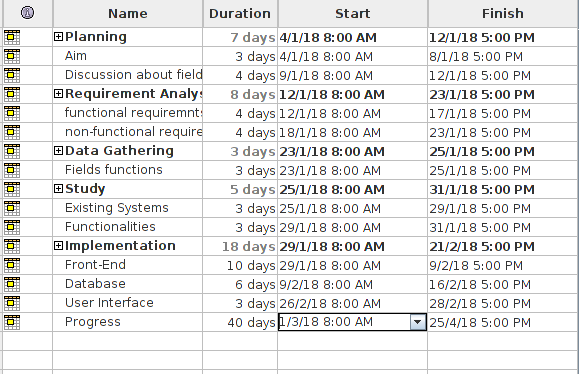
\includegraphics[scale=.74]{input/images/chart2.png}
	\caption{Plan}
\end{figure}
\newpage
\section{Progress}

A Gantt chart is a type of bar chart that illustrates a project schedule. This chart lists the tasks to be performed on the vertical axis, and time intervals on the horizontal axis.\\\\
A Gantt chart is a graphical depiction of a project schedule. A Gantt chart is a type of bar chart that shows the start and finish dates of several elements of a project that include resources, milestones, tasks and dependencies. \\\\


 \begin{figure}[h!]
	\centering 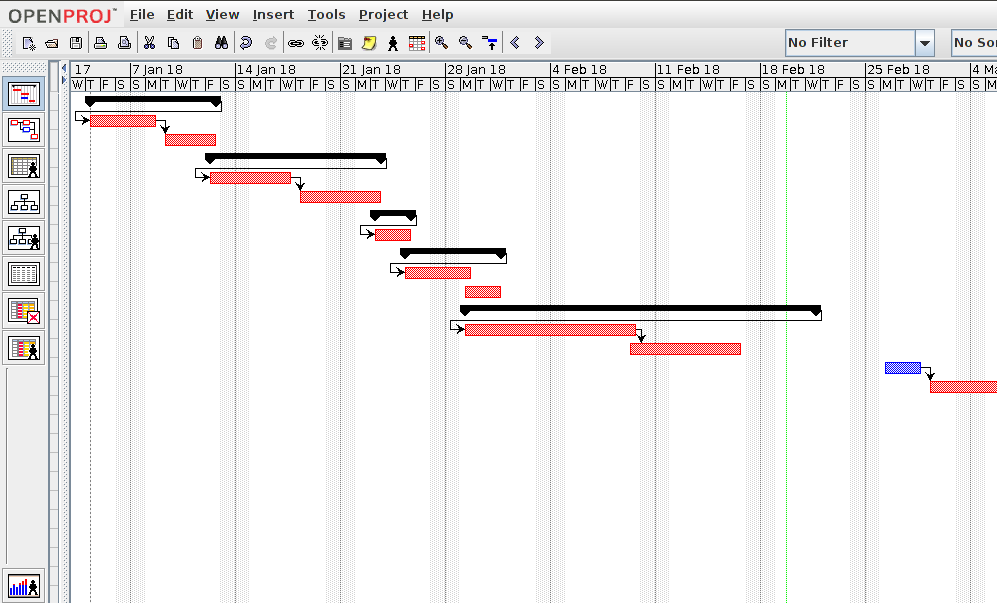
\includegraphics[scale=.43]{input/images/chart1.png}
	\caption{Gantt Chart}
\end{figure}


Gantt charts are most commonly used for tracking project schedules. For this it is useful to be able to show additional information about the various tasks or phases of the project, for example how the tasks \\
Gantt charts may be simple versions created on graph paper or more complex automated versions created using project management applications.